%%%%%%%%%%%%%%%%%%%%%%%%%%%%%%%%%%%%%%%%%
% Beamer Presentation
% LaTeX Template
% Version 1.0 (10/11/12)
%
% This template has been downloaded from:
% http://www.LaTeXTemplates.com
%
% License:
% CC BY-NC-SA 3.0 (http://creativecommons.org/licenses/by-nc-sa/3.0/)
%
%%%%%%%%%%%%%%%%%%%%%%%%%%%%%%%%%%%%%%%%%

%----------------------------------------------------------------------------------------
%	PACKAGES AND THEMES
%----------------------------------------------------------------------------------------

\documentclass[aspectratio=169]{beamer}
\usepackage[portuges]{babel}
\usepackage[utf8]{inputenc}
\usepackage[alf]{abntex2cite}	
\usepackage[portuguese, linesnumbered, vlined, titlenumbered, ruled]{algorithm2e}
\SetKwRepeat{Registro}{registro \{}{\}}%
\usepackage{beamerthemesplit}
\usepackage{multirow}
\usepackage{scalefnt}

% Macro que faz com que a numeracao de diferentes algoritmos continue de onde parou
\newcommand{\rememberlines}{\xdef\rememberedlines{\number\value{AlgoLine}}}
\newcommand{\resumenumbering}{\setcounter{AlgoLine}{\rememberedlines}}

% The Beamer class comes with a number of default slide themes
% which change the colors and layouts of slides. Below this is a list
% of all the themes, uncomment each in turn to see what they look like.

%\usetheme{default}
%\usetheme{AnnArbor}
%\usetheme{Antibes}
%\usetheme{Bergen}
%\usetheme{Berkeley}
%\usetheme{Berlin}
%\usetheme{Boadilla}
%\usetheme{CambridgeUS}
%\usetheme{Copenhagen}
%\usetheme{Darmstadt}
%\usetheme{Dresden}
%\usetheme{Frankfurt}
%\usetheme{Goettingen}
%\usetheme{Hannover}
%\usetheme{Ilmenau}
%\usetheme{JuanLesPins}
%\usetheme{Luebeck}
\usetheme{Madrid}
%\usetheme{Malmoe}
%\usetheme{Marburg}
%\usetheme{Montpellier}
%\usetheme{PaloAlto}
%\usetheme{Pittsburgh}
%\usetheme{Rochester}
%\usetheme{Singapore}
%\usetheme{Szeged}
%\usetheme{Warsaw}

% As well as themes, the Beamer class has a number of color themes
% for any slide theme. Uncomment each of these in turn to see how it
% changes the colors of your current slide theme.

%\usecolortheme{albatross}
%\usecolortheme{beaver}
%\usecolortheme{beetle}
%\usecolortheme{crane}
\usecolortheme{dolphin}
%\usecolortheme{dove}
%\usecolortheme{fly}
%\usecolortheme{lily}
%\usecolortheme{orchid}
%\usecolortheme{rose}
%\usecolortheme{seagull}
%\usecolortheme{seahorse}
%\usecolortheme{whale}
%\usecolortheme{wolverine}

%\setbeamertemplate{footline} % To remove the footer line in all slides uncomment this line
%\setbeamertemplate{footline}[page number] % To replace the footer line in all slides with a simple slide count uncomment this line

%\setbeamertemplate{navigation symbols}{} % To remove the navigation symbols from the bottom of all slides uncomment this line


\usepackage{graphicx} % Allows including images
\usepackage{booktabs} % Allows the use of \toprule, \midrule and \bottomrule in tables

%----------------------------------------------------------------------------------------
%	TITLE PAGE
%----------------------------------------------------------------------------------------
\title[Árvores B]{Algoritmos e Estrutura de Dados}
\subtitle{Árvores B}
\author[Frederico Santos de Oliveira]{prof. Frederico Santos de Oliveira}
\institute[UFMT]{Universidade Federal de Mato Grosso\\ Faculdade de Engenharia}
\date{}

\begin{document}

%%%%%%%%%%%%%%%%%%%%%%%%%%%%%%%%%%%%%%%%%%%%%%%%%%%%%%%%%%%%%%%%%%%%%%%%%%%%%%%%%%%%%%%%%%%%%%%%%%%%%%%%%
\begin{frame}
\titlepage % Print the title page as the first slide

\begin{figure}[!h]
  \centering
   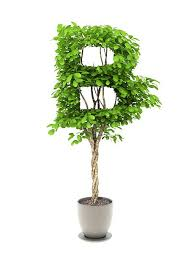
\includegraphics[width=80pt]{imagens/introducao.jpg}
  \label{fig_introducao}
\end{figure}
\end{frame}

%%%%%%%%%%%%%%%%%%%%%%%%%%%%%%%%%%%%%%%%%%%%%%%%%%%%%%%%%%%%%%%%%%%%%%%%%%%%%%%%%%%%%%%%%%%%%%%%%%%%%%%%%

\begin{frame}
\frametitle{Roteiro} % Table of contents slide, comment this block out to remove it
\tableofcontents % Throughout your presentation, if you choose to use \section{} and \subsection{} commands, these will automatically be printed on this slide as an overview of your presentation
\end{frame}

%----------------------------------------------------------------------------------------
%	PRESENTATION SLIDES
%----------------------------------------------------------------------------------------

%%%%%%%%%%%%%%%%%%%%%%%%%%%%%%%%%%%%%%%%%%%%%%%%%%%%%%%%%%%%%%%%%%%%%%%%%%%%%%%%%%%%%%%%%%%%%%%%%%%%%%%%%
\section{Objetivos}
%%%%%%%%%%%%%%%%%%%%%%%%%%%%%%%%%%%%%%%%%%%%%%%%%%%%%%%%%%%%%%%%%%%%%%%%%%%%%%%%%%%%%%%%%%%%%%%%%%%%%%%%%

\begin{frame}
\frametitle{Objetivos}
Esta aula tem como objetivos:
\begin{enumerate}
\item Apresentar os conceitos básicos sobre árvores B;
\item Exemplificar os algoritmos de manipulação de árvores B por meio de pseudo-códigos.
\end{enumerate}
\end{frame}

%%%%%%%%%%%%%%%%%%%%%%%%%%%%%%%%%%%%%%%%%%%%%%%%%%%%%%%%%%%%%%%%%%%%%%%%%%%%%%%%%%%%%%%%%%%%%%%%%%%%%%%%%
\section{Introdução}
%%%%%%%%%%%%%%%%%%%%%%%%%%%%%%%%%%%%%%%%%%%%%%%%%%%%%%%%%%%%%%%%%%%%%%%%%%%%%%%%%%%%%%%%%%%%%%%%%%%%%%%%%

\begin{frame}{Introdução}
\begin{itemize}
 \item O acesso a disco envolve um posicionamento da cabeça do disco, além da transferência de dados propriamente ditos. 
 \item O posicionamento depende do tempo de rotação do disco que é da ordem de 8 mili-segundos. 
\end{itemize} 
\begin{figure}[!h]
  \centering
   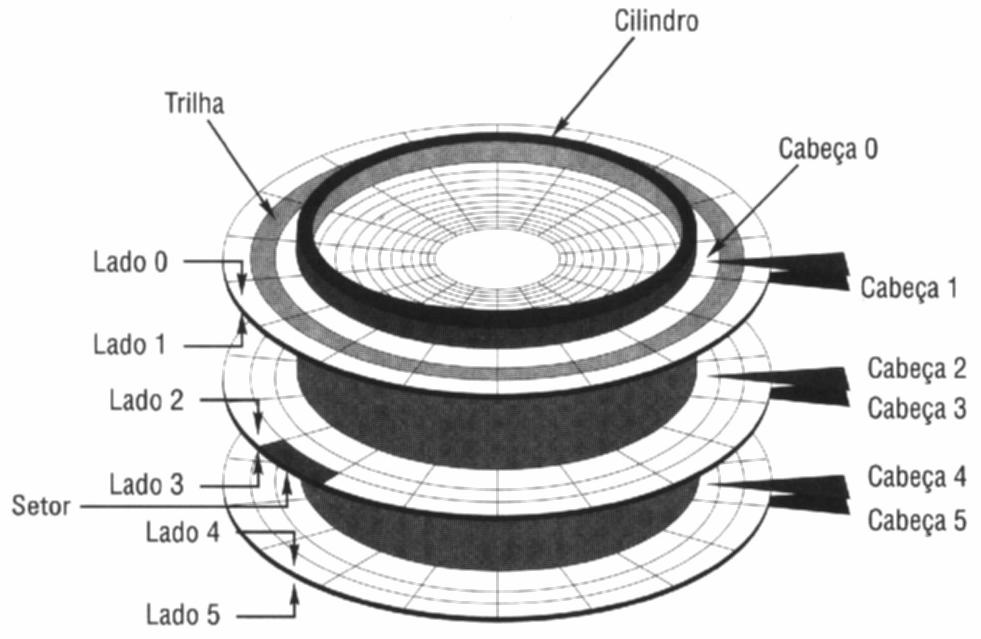
\includegraphics[width=200pt]{imagens/disco_rigido1.jpg}
  \label{fig_disco_rigido1}
\end{figure} 
\end{frame}

%%%%%%%%%%%%%%%%%%%%%%%%%%%%%%%%%%%%%%%%%%%%%%%%%%%%%%%%%%%%%%%%%%%%%%%%%%%%%%%%%%%%%%%%%%%%%%%%%%%%%%%%%

\begin{frame}{Introdução}
\begin{itemize}
 \item Um acesso a disco leva tipicamente 10 a 15 milisegundos, o que é considerável em comparação com o tempo de acesso à memória primária (RAM), da ordem de 100 nano-segundos. 
 \item No tempo para acessar uma vez o disco, podemos fazer cerca de 100.000 acessos à memória.
\end{itemize}
\begin{figure}[!h]
  \centering
   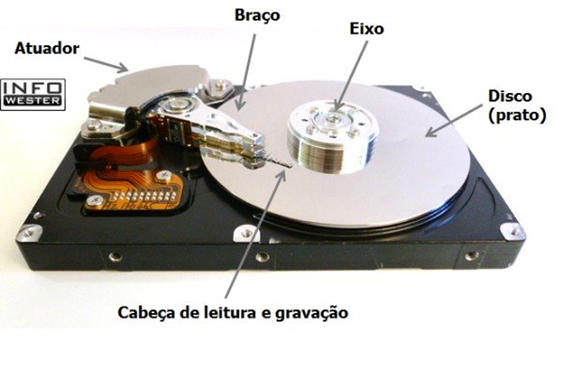
\includegraphics[width=150pt]{imagens/disco_rigido2.png}
  \label{fig_disco_rigido2}
\end{figure} 
\end{frame}

%%%%%%%%%%%%%%%%%%%%%%%%%%%%%%%%%%%%%%%%%%%%%%%%%%%%%%%%%%%%%%%%%%%%%%%%%%%%%%%%%%%%%%%%%%%%%%%%%%%%%%%%%
\section{Motivação}
%%%%%%%%%%%%%%%%%%%%%%%%%%%%%%%%%%%%%%%%%%%%%%%%%%%%%%%%%%%%%%%%%%%%%%%%%%%%%%%%%%%%%%%%%%%%%%%%%%%%%%%%%

\begin{frame}{Introdução}{Motivação}
\begin{itemize}
\item Árvores binárias de Busca (balanceadas ou não) não são adequadas para buscar dados na memória secundária.
\begin{itemize}
\item Para acessar cada nodo da árvore é necessário fazer uma consulta ao disco rígido.
\item Portanto, ao realizar uma consulta, seria necessário aguardar alguns milisegundos.
\end{itemize}
\item Mesmo em árvores AVL, uma grande quantidade de chaves pode requerer um número excessivo de acessos a disco rígido. 
\begin{itemize}
\item Em uma árvore AVL, com $n = 10^6$, o valor de $\log_2 n \approx 10$, ou seja, seriam necessários aproximadamente 20 acessos a disco rígido, o que é altamente custoso.
\end{itemize}
\end{itemize}
\end{frame}

%%%%%%%%%%%%%%%%%%%%%%%%%%%%%%%%%%%%%%%%%%%%%%%%%%%%%%%%%%%%%%%%%%%%%%%%%%%%%%%%%%%%%%%%%%%%%%%%%%%%%%%%%

\begin{frame}{Introdução}{Motivação}
\begin{itemize}
\item Uma operação de acesso ao disco é cara, portanto é necessário consultar uma quantidade maior de dados.
\begin{itemize}
\item Vetores são armazenados em posições contíguas no disco rígido, portanto em um único acesso todo o vetor é carregado para a memória.
\end{itemize}
\item Diante disso, \cite{Bayer1970} criaram as Árvores B, em que cada nodo armazena um vetor de elementos.
\begin{itemize}
\item O nome "Árvore B" é um mistério.
\item Conjectura-se que seja ``B'' de ``B''ayer, ou de ``B''alanceada ou ainda de ``B''oeing, a companhia onde trabalhavam os dois autores.
\end{itemize}
\item Nas árvores B, um nodo pode conter centenas de chaves, e é chamado de {\bf página}.
\end{itemize}
\end{frame}

%%%%%%%%%%%%%%%%%%%%%%%%%%%%%%%%%%%%%%%%%%%%%%%%%%%%%%%%%%%%%%%%%%%%%%%%%%%%%%%%%%%%%%%%%%%%%%%%%%%%%%%%%
\section{Definição}
%%%%%%%%%%%%%%%%%%%%%%%%%%%%%%%%%%%%%%%%%%%%%%%%%%%%%%%%%%%%%%%%%%%%%%%%%%%%%%%%%%%%%%%%%%%%%%%%%%%%%%%%%

\begin{frame}{Árvores B}{Definição}
\begin{itemize}
\item Nas Árvores B existe uma quantidade máxima e mínima de chaves que podem ser armazenadas em um nodo.
\begin{itemize}
\item  Esses limites são definidos de acordo com uma {\bf ordem}, explicada a seguir.
\end{itemize}
\item Devido à sua estrutura, todos os nodos folhas permanecem no mesmo nível, que é a altura $h$ da árvore.
\begin{itemize}
\item Diferentemente das outras árvores estudadas, as Árvores B crescem para cima.
\end{itemize}
\item Além disso, é garantido que qualquer nodo em uma Árvore B possui pelo menos 50\% de quantidade máxima de chaves.
\end{itemize}
\end{frame}

%----------------------------------------------------------------------------------------
\subsection{Ordem}
%----------------------------------------------------------------------------------------

\begin{frame}{Introdução}{Ordem}
\begin{itemize}
\item Considere {\bf ordem} um inteiro $t \geq 2$, de forma que representa o \underline{grau} (quantidade de filhos) mínimo da árvore. 
\item A ordem de uma Árvore B define a quantidade mínima e máxima de chaves em uma página.
\begin{itemize}
\item Qualquer página (exceto a raiz) deve ter no mínimo {\bf $t-1$} chaves. 
\begin{itemize}
\item Ou seja, deve possuir no mínimo {\bf $t$} filhos.
\end{itemize}
\item Toda página deve conter no máximo {\bf $2t-1$} chaves. 
\begin{itemize}
\item Portanto, toda página interna tem no máximo {\bf $2t$} filhos.
\end{itemize}
\end{itemize}
\item Quantidade $n$ de chaves: $t-1 \leq n \leq 2t-1$.
\item Quantidade $m$ de filhos: $t \leq m \leq 2t$
\end{itemize}
\end{frame}

%----------------------------------------------------------------------------------------

\begin{frame}{Árvores B}{Exemplo}
Exemplo de uma Árvore B, de ordem $t=2$, denominada Árvore 2-3-4:
\begin{figure}[!h]
  \centering
   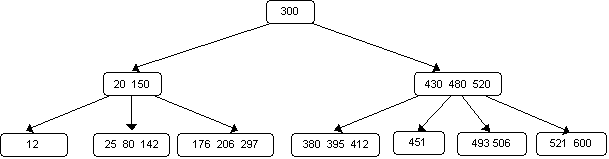
\includegraphics[width=300pt]{imagens/exemplo1-arvore-b.png}
  \label{fig_exemplo1-arvore-b}
\end{figure} 
\begin{itemize}
 \item Toda página interna possui $1\leq n \leq 3$ chaves.
 \item Toda página interna possui $2\leq m \leq 4$ filhos, daí o nome Árvore 2-3-4.
 \item Todos as páginas folhas estão na mesma altura na árvore.
\end{itemize}
\end{frame}

%----------------------------------------------------------------------------------------
\subsection{Estrutura Nodo}
%----------------------------------------------------------------------------------------

\begin{frame}{Introdução}{Estrutura Nodo}
A estrutura de dados {\bf nodo} de uma Árvore B possui quatro campos:
 \begin{enumerate}
 \item O total de chaves $n$ atualmente armazenadas no nodo.
 \item Um vetor, denominado $key$, de tamanho $n$, em que as chaves são armazenadas em ordem não-decrescente:
 \begin{equation}
  key_1 \leq key_2 \leq ... \leq key_n. \nonumber
 \end{equation}
 \item Um valor booleano, denominado $folha$, que indica se é folha ou um nodo interno.
 \item Um vetor contendo $n+1$ ponteiros, $c_1, c_2, ..., c_{n+1}$, para os filhos.
 \begin{itemize}
 \item Caso o nodo seja folha, seus ponteiros apontam para NULL.
 \end{itemize}
 \end{enumerate}
\begin{figure}[!h]
  \centering
   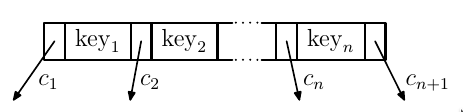
\includegraphics[width=150pt]{imagens/estrutura_nodo.png}
  \label{fig_estrutura_nodo}
\end{figure} 
\end{frame}

%----------------------------------------------------------------------------------------

\begin{frame}[fragile]{Árvore Binária}{Estrutura Nodo}
\begin{algorithm}[H]
\caption{Nodo} 
\label{Nodo}
\Inicio{
 \Registro{Nodo}{
    Vetor Inteiro: key[1..2t-1]; \CommentSty{// Vetor de chaves.}\\
    Vetor Ponteiro Nodo: c[1..2t]; \CommentSty{// Vetor de ponteiros.} \\
    Inteiro: n; \CommentSty{// Quantidade de chaves armazenadas.} \\
    Booleano: folha; \CommentSty{// Indica se o nodo é folha.}
  }
}
\end{algorithm} 
\end{frame}

%----------------------------------------------------------------------------------------

\begin{frame}{Árvores B}{Ordenação}
\begin{itemize}
\item Assim como nas árvores binárias, nas Árvores B cada chave $key_i$ possui filhos à esquerda (localizados em $c_i$) e filhos à direita (localizados em $c_{i+1}$).
\begin{figure}[!h]
  \centering
   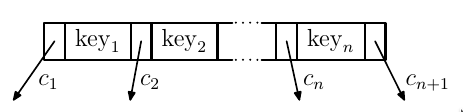
\includegraphics[width=150pt]{imagens/estrutura_nodo.png}
  \label{fig_estrutura_nodo1}
\end{figure} 
\item Considere $c_i.k$, qualquer chave pertencente à $c_i$.
\begin{itemize}
\item Toda chave $c_i.k$  armazenada no filho da esquerda $c_i$ satisfaz $c_i.k \leq key_i$.
\item De forma análoga, toda chave $c_{i+1}.k$ armazenada no filho da direita $c_{i+1}$ satisfaz $key_i \leq c_{i+1}.k \leq key_{i+1}$.
\end{itemize}
\item Dessa forma, temos
\end{itemize}
\begin{equation}
 c_1.k \leq key_1 \leq c_2.k \leq key_2 \leq c_3.k \leq ... \leq key_n \leq c_{n+1}.k. \nonumber 
\end{equation}
\end{frame}

%----------------------------------------------------------------------------------------

\begin{frame}{Árvores B}{Ordenação}
\begin{figure}[!h]
\centering
   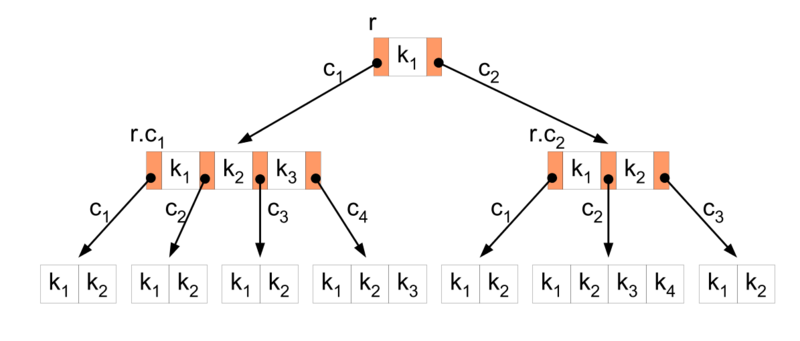
\includegraphics[width=300pt]{imagens/exemplo2-arvore-b.png}
  \label{fig_exemplo2-arvore-b}
\end{figure} 
\end{frame}

%----------------------------------------------------------------------------------------
\subsection{Altura}
%----------------------------------------------------------------------------------------

\begin{frame}{Introdução}{Altura}
Uma Árvore B de altura 3 contém um número {\bf mínimo} possível de chaves.
\begin{figure}[!h]
\centering
   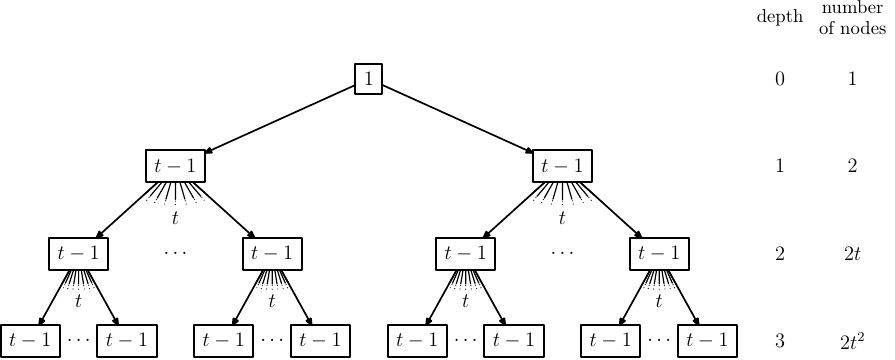
\includegraphics[width=300pt]{imagens/altura.png}
  \label{fig_altura}
\end{figure}
Conforme mostrado na figura, cada nodo possui no mínimo $t-1$ chaves, exceto a raiz.
\end{frame}

%----------------------------------------------------------------------------------------

\begin{frame}{Introdução}{Altura}
\begin{itemize}
\item Analisando a quantidade de nodos:
\begin{itemize}
\item No nível $1$, tem-se $2t^{0}$ nodos.
\item No nível $2$, tem-se $2t^{1}$ nodos.
\item No nível $3$, tem-se $2t^{2}$ nodos.
\item De forma análoga, no nível $i$, tem-se $2 t^{i-1}$ nodos.
\end{itemize}
\item Portanto, a árvore possui um total de $1 + \sum_{i=1}^h 2 t^{i-1}$ nodos.
\begin{itemize}
\item O valor "$+1$" refere-se a raiz.
\end{itemize}
\end{itemize}
\end{frame}

%----------------------------------------------------------------------------------------

\begin{frame}{Introdução}{Altura}
\begin{itemize}
\item Verificamos que trata-se de uma PG (Progressão Geométrica).
\begin{itemize}
\item $2t^{0} + 2t^{1} + 2t^{2} + ...  + 2t^{h-1}$.
\end{itemize} 
\item Essa PG possui $a_1 = 2$, a razão $q=t$, e a quantidade de elementos $n=h$, em que $h$ é a altura da árvore. 
\item Com isso, podemos calcular o {\bf total de nodos} $S_n$ da seguinte forma:
\begin{eqnarray}
S_n &=& \frac{ a_1 ( q^n - 1)} {q - 1} \nonumber \\
    &=& \frac{ 2 ( t^h - 1)} {t - 1}.\nonumber
\end{eqnarray}
\end{itemize}
\end{frame}


%----------------------------------------------------------------------------------------

\begin{frame}{Introdução}{Altura}
Exceto a raiz, cada nodo armazena no mínimo $t-1$ chaves. Portanto, o {\bf total de chaves} $n$ da árvore é igual a $(t-1)$ vezes o total de nodos mais a chave na raiz:
\begin{eqnarray}
n &\geq& 1 + (t-1) S_n \nonumber \\
  &\geq& 1 + (t-1) \frac{ 2 (t^h - 1)} {t - 1} \geq  2 t^h - 1 \nonumber
\end{eqnarray}
A altura da árvore em função da quantidade de chaves pode ser obtida da seguinte forma:
\begin{eqnarray}
2 t^h - 1 &\leq & n \nonumber \\
t^h &\leq & \frac{n + 1}{2} \nonumber \\
\log_t t^h &\leq & \log_t (\frac{n + 1}{2}) \nonumber \\
 h &\leq &\log_t (\frac{n + 1}{2}) \nonumber
\end{eqnarray}
\end{frame}

%----------------------------------------------------------------------------------------

\begin{frame}{Introdução}{Altura}
\begin{itemize}
\item O número de acessos ao disco é proporcional à altura da Árvore B.
\item No pior caso, referente à altura da Árvore B, é
\begin{equation}
 h \leq \log_t \frac{n+1}{2} \approx O(\log_t n).\nonumber
\end{equation}
\end{itemize}
\end{frame}

%----------------------------------------------------------------------------------------

\begin{frame}{Introdução}{Altura}
 As principais vantagens da Árvore B em relação às outras árvores são:
\begin{itemize}
\item A base do logaritmo, $t$, deve ser um valor grande, o que reduz o custo das operações.
\item Árvores B reduzem o número de nodos examinados nas operações (busca, inserção e remoção) em um fator $\log t$.
\item Dessa forma, o número de acessos ao disco é reduzido substancialmente.
\end{itemize}
\end{frame}

% 
% 
% \begin{frame}{Introdução}{Definição}
% \begin{itemize}
% \item Uma Árvore B com raiz em $r$ possui as seguintes propriedades:
% \begin{itemize}
%  \item Cada página contém no máximo 2b chaves.
%  \item Cada página, exceto a página raiz, contém no mínimo b chaves.
%  \item Uma página com m chaves $k_1 < k_2 < ... < k_m$ possui $m + 1$ ponteiros $p_0 , p_1 , . . . p_m$. 
%  \item Só há duas situações possíveis:
%  \begin{enumerate}
%  \item A página é uma folha e não tem filhos: todos os ponteiros $p_i$ , $0 \leq i \leq m$ apontam para NULL.
%  \item A página não é folha e possui $m + 1$ filhos apontados por $pi$ , $0 \leq i \leq m$. Nenhum ponteiro aponta para NULL.
%  \end{enumerate}
% \end{itemize}
% \end{itemize}
% \end{frame}
% 
% \begin{frame}{Introdução}{Definição}
% \begin{itemize}
%  \item Se a página não é uma folha:
%  \begin{itemize}
%  \item Para toda chave $k$ na subárvore apontada por $p_0$, $k < k_1$.
%  \item Para toda chave $k$ na subárvore apontada por $p_m$, $k > k_m$.
%  \item Para toda chave $k$ na subárvore apontada por $p_i$, $1 \leq i < m, k_i < k < k_{i+1}$.
%  \item Todas as páginas folhas aparecem no mesmo nível.
%  \end{itemize}
%  \end{itemize}
% \begin{figure}[!h]
%   \centering
%    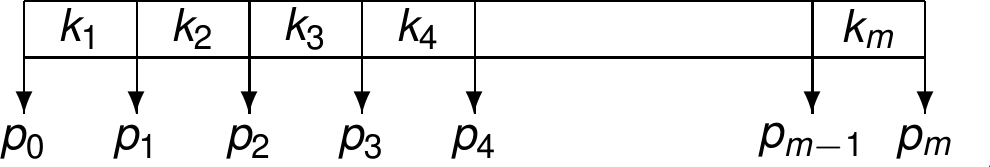
\includegraphics[width=150pt]{imagens/estrutura_pagina.png}
%   \label{fig_estrutura_pagina}
% \end{figure} 
% \end{frame}

%----------------------------------------------------------------------------------------
{\section{Operações Básicas}
%----------------------------------------------------------------------------------------

\begin{frame}{Operações Básicas}
A seguir, as operações básicas a serem realizadas sobre Árvores B:
 \begin{itemize}
 \item ArvoreB-Criar
 \item ArvoreB-Busca
 \item ArvoreB-Inserir
 \item ArvoreB-Remover
\end{itemize}
\end{frame}

%----------------------------------------------------------------------------------------

\begin{frame}{Operações Básicas}
 Conveções:
\begin{itemize}
\item A raiz de uma Árvore B sempre está na memória principal (DISK-READ na raiz nunca será necessário).
\item Qualquer nodo passado como parâmetro deve ter uma operação DISK-READ realizada sobre ele, a fim de ler os dados do disco.
\item Sempre que um nodo for alterado, deve ter uma operação DISK-WRITE realizada sobre ele, a fim de salvar os dados no disco.
\item Todos os procedimentos apresentados são algoritmos {\bf top-down}, iniciando na raiz da árvore.
\end{itemize}
\end{frame}

%----------------------------------------------------------------------------------------
\subsection{Criar}
%----------------------------------------------------------------------------------------

\begin{frame}{CriaÁrvore}{Pseudocódigo}
% \scalebox{0.8}{
\begin{algorithm}[H]
\caption{ArvoreB-Criar} 
\label{B-Tree-Create}
\Entrada{Ponteiro $T$ para a árvore.}
\Inicio{
  novo $\leftarrow$ ALOCA\_NODO() \\
  novo.folha $\leftarrow$ TRUE \\
  novo.n $\leftarrow$ 0 \\
  DISK\_WRITE(novo) \\
  T.raiz $\leftarrow$ novo
}
\end{algorithm}
\tiny{Adaptado de \cite{Cormen2012}.}
% }  
\begin{itemize}
 \item ALOCA\_NODO() aloca uma página no disco de modo a ser usada como um novo nodo.
 \item Requer $O(1)$ operações no disco e tempo de processador $O(1)$.
\end{itemize}
\end{frame}

%----------------------------------------------------------------------------------------
\subsection{Busca}
%----------------------------------------------------------------------------------------

\begin{frame}{Busca}
\begin{itemize}
 \item A busca de uma dada chave $k$ numa árvore B é análoga à busca na árvore binária de busca. 
 \item A busca começa pela página raiz $r$. 
 \item É usual manter a raiz sempre na memória, evitando um acesso ao disco. 
\end{itemize}
\end{frame}

%----------------------------------------------------------------------------------------

\begin{frame}{Busca}
\begin{itemize}
 \item Estando em uma página da Árvore B, procedemos assim:
\begin{enumerate}
\item Busca-se $k$ em $r$, usando um método de busca sequencial ou busca binária, dependendo do valor de $t$. Para pequenos valores de $t$, busca sequencial já basta.
\item Se $k$ estiver em $r$, então retorna o nodo $r$ e a posição de $k$ na página.
\item Se $k < key[1]$, então realiza a busca recursivamente na página apontada por $c[1]$ .
\item Se $key[i] < k < key[i+1]$, então continua a busca na página apontada por $c[i+1]$.
\item Se $k > key[n]$, então continua a busca na página apontada por $c[n+1]$.
\end{enumerate}
\item Pode-se ver que a busca leva tempo $O(\log_t n)$, onde $t$ é a ordem da árvore B e $n$ é o número total de chaves.
\end{itemize}
\end{frame}

%----------------------------------------------------------------------------------------

\begin{frame}{Busca}{Pseudocódigo}
\scalebox{0.95}{
\begin{algorithm}[H]
\caption{ArvoreB-Busca} 
\label{B-Tree-Search}
\Entrada{Ponteiro para a raiz $r$, chave $k$ a ser buscada na árvore.}
\Saida{O nodo que contém $k$ ou NULL caso não encontre.}
\Inicio{
  i$\leftarrow$ 1 \\
  \Enqto{($i \leq r.n$) AND ($k > r.key[i]$)} {
    $i \leftarrow i + 1$ \\ 
  }
  \Se {($i\leq r.n$) AND ($k = r.key[i]$)} {
    \Retorna (r, i)
  }
  \Se {(r.folha)} {
    \Retorna NULL
  }
  \Senao { 
    DISK\_READ($r.c_i$) \\
    \Retorna ArvoreB-Busca($r.c[i]$, k)
  }
}
\end{algorithm}
}  
\tiny{Adaptado de \cite{Cormen2012}}.
\end{frame}

%----------------------------------------------------------------------------------------

\begin{frame}{Busca}
\begin{itemize}
 \item Número de páginas do disco acessadas por ArvoreB-Busca
 \begin{equation}
  \Theta(h) = \Theta(\log_t n) \nonumber
 \end{equation}
 \item Tempo de execução do laço {\bf enquanto} (linhas 3-4) dentro de cada nodo é $O(t)$.
 \item Portanto o tempo total de execução é:
 \begin{equation}
  O(t \times h) = O(t \log_t n) \nonumber
 \end{equation}
\end{itemize}
\end{frame}

%----------------------------------------------------------------------------------------
\subsection{Inserção}
%----------------------------------------------------------------------------------------

\begin{frame}{Inserção}
\begin{itemize}
 \item Para inserir uma nova chave $x$ numa árvore B de ordem $t$, existem dois casos a serem considerados.
 \item  A seguir os passos necessários:
 \begin{itemize}
 \item Primeiro localizamos a página folha onde será feita a inserção.
 \item Verificamos quantas chaves já estão na página antes de adicionar a chave $k$ na mesma.
 \item {\bf Caso 1}: Se a página contém menos que $2t-1$ chaves, então basta inserir a nova chave $k$ na página.
 \end{itemize}
\end{itemize}
\end{frame}

%----------------------------------------------------------------------------------------

\begin{frame}{Inserção}
\begin{itemize}
 \item {\bf Caso 2}: Se a página contém exatamente $2t-1$ chaves, então é necessário realizar a sua divisão:
 \begin{itemize}
 \item Inclua a nova chave $k$, em ordem não decrescente, na página em questão. Dessa forma, a página terá $2t$ chaves
 \item Em seguida, realiza-se a divisão (ou cisão) da página em duas.
 \item O elemento do meio (posição $t$) é inserido, recursivamente, na página pai.
 \item Alocamos as primeiras $t-1$ chaves numa página e as últimas $t$ chaves noutra página.
 \end{itemize} 
\end{itemize}
\begin{figure}[!h]
\centering
   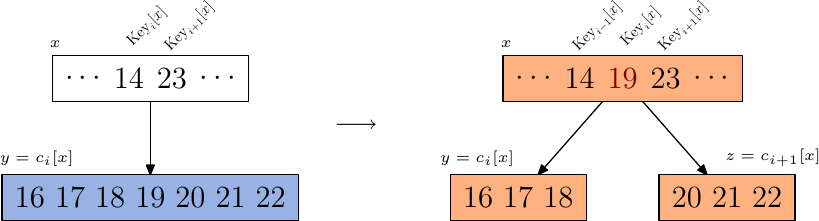
\includegraphics[width=300pt]{imagens/divisao.png}
  \label{fig_divisao}
\end{figure} 
\end{frame}

%----------------------------------------------------------------------------------------

\begin{frame}{Inserção}{Divisão}
A seguir, os passos necessários para realizar a divisão de um nodo:
\begin{itemize}
\item Considere dividir o nodo $y$ filho de $x$, localizado na posição $i$.
\begin{itemize}
\item Ou seja, $y = x.c[i]$.
\end{itemize}
\item Para isso, deve-se:
\begin{itemize}
\item Alocar um novo nodo $z$.
\item Copiar as chaves de $y$ para $z$.
\item Copiar os ponteiros de $y$ para $z$.
\item Mover o elemento no meio de $y$ para $x$.
\end{itemize}
\end{itemize}
\begin{figure}[!h]
\centering
   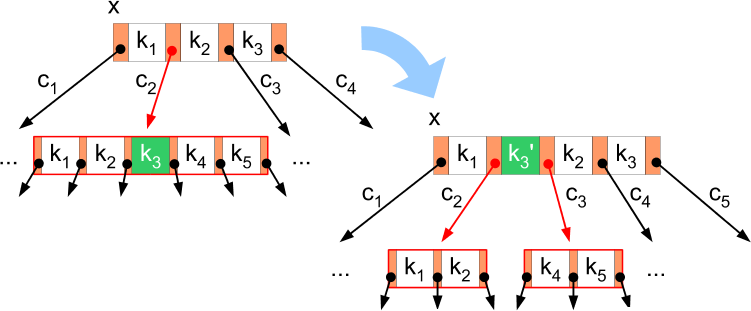
\includegraphics[width=230pt]{imagens/exemplo_divide_filho.png}
  \label{fig_exemplo_divide_filho}
\end{figure} 
\end{frame}


%----------------------------------------------------------------------------------------

\begin{frame}{Divisão}{Pseudocódigo}
\scalebox{0.95}{
\begin{algorithm}[H]
\caption{ArvoreB-Divide-Filho} 
\label{B-Tree-Split-CHild}
\Entrada{Um nodo interno não-cheio $x$, um índice $i$, um nodo cheio $y$ filho de $x$, tal que $y=x.c_i$.}
\Inicio{  
  z $\leftarrow$ ALOCA\_NODO() \label{divide_filho_aloca_z_inicio}\\
  z.folha $\leftarrow$ y.folha \\
  z.n $\leftarrow$ t-1 \label{divide_filho_aloca_z_fim} \\
  \Para {($j\leftarrow 1$ \textrm{ até } t-1)} { \label{divide_filho_aloca_copia_inicio}
    $z.key[j] \leftarrow y.key[j+t]$ \\
  }\label{divide_filho_aloca_copia_fim}
  \Se {(NOT(y.folha))} { \label{divide_filho_aloca_copia_c_inicio}
    \Para {($j \leftarrow 1$ \textrm{ até } t)} {
      $z.c[j] \leftarrow y.c[j+t]$ \\     
    }
  } \label{divide_filho_aloca_copia_c_fim}
  y.n $\leftarrow$ t-1 \label{divide_filho_atualiza_y} \\
  \rememberlines
}
\end{algorithm}
}
\tiny{Adaptado de \cite{Cormen2012}.}  
\end{frame}

%----------------------------------------------------------------------------------------

\begin{frame}{Divisão}{Pseudocódigo}
Vamos analisar o algoritmo ArvoreB-Divide-Filho.
\begin{itemize}
 \item Deseja-se dividir o nodo $y$, cujo pai é $x$.
 \begin{itemize}
  \item O nodo $y$ está cheio e possui $2t-1$ chaves.
 \end{itemize}
 \item Primeiramente cria-se um novo nodo, denominado $z$, linhas \ref{divide_filho_aloca_z_inicio} a \ref{divide_filho_aloca_z_fim}.
 \begin{itemize}
 \item $z$ será folha se $y$ for folha.
 \item $z$ terá a quantidade mínima de chaves, que é $t-1$.
 \end{itemize}
 \item Em seguida, copias as chaves de $y$  para $z$, linhas \ref{divide_filho_aloca_copia_inicio} a \ref{divide_filho_aloca_copia_fim}.
 \begin{itemize}
 \item As primeiras $t-1$ chaves permanecerão em $y$.
 \item O elemento na posição $t$ de $y$ será movido para o pai $x$.
 \item As $t-1$ chaves restantes serão copiadas para $z$.
\end{itemize}
 \item Copia os ponteiros de $y$  para $z$, linhas \ref{divide_filho_aloca_copia_c_inicio} a \ref{divide_filho_aloca_copia_c_fim}.
 \begin{itemize}
 \item Copia $t$ ponteiros de $y$ para $z$ a partir da posição $t$.
\end{itemize}
\item Dessa forma, deve-se atualizar a quantidade de chaves de $y$ (linha \ref{divide_filho_atualiza_y}).
\end{itemize}
\end{frame}

%----------------------------------------------------------------------------------------


\begin{frame}{Divisão}{Pseudocódigo}
\scalebox{0.95}{
\begin{algorithm}[H]
\caption{ArvoreB-Divide-Filho (continuação)} 
\label{B-Tree-Create2}
\resumenumbering
\Inicio{
  \Para {($j\leftarrow x.n+1$ \textrm{ descendo até } $i+1$)} { \label{divide_filho_move_x_inicio}
    $x.c[j+1] \leftarrow x.c[j]$ \\
  } \label{divide_filho_move_x_fim}
  $x.c[i+1] \leftarrow z$ \label{divide_filho_atualiza_filho_z} \\
  \Para {($j\leftarrow x.n$ \textrm{ descendo até } $i$)} { \label{divide_filho_move_chave_x_inicio}
    $x.key[j+1] \leftarrow x.key[j]$ \\
  } \label{divide_filho_move_chave_x_fim}
  $x.key[i] \leftarrow y.key[t]$ \label{divide_filho_adiciona_chave_x} \\ 
  $x.n \leftarrow x.n + 1$ \label{divide_filho_atualiza_x} \\
  DISK\_WRITE(y)\\
  DISK\_WRITE(z)\\
  DISK\_WRITE(x)\\
}
\end{algorithm}
}
\tiny{Adaptado de \cite{Cormen2012}.}
\end{frame}

%----------------------------------------------------------------------------------------

\begin{frame}{Divisão}{Pseudocódigo}
Vamos analisar a continuação do algoritmo ArvoreB-Divide-Filho.
\begin{itemize}
 \item Move os ponteiros de $x$ para a direita, linhas \ref{divide_filho_move_x_inicio} a \ref{divide_filho_move_x_fim}.
 \item Adiciona $z$ como filho de $x$ na posição $i+1$, linha \ref{divide_filho_atualiza_filho_z}.
 \item Move as chaves de $x$ para a direita, linhas \ref{divide_filho_move_chave_x_inicio} a \ref{divide_filho_move_chave_x_fim}.
 \item Insere o elemento que encontra-se no meio de $y$ em	 $z$, linha \ref{divide_filho_adiciona_chave_x}.
 \item Atualiza o total de nodos armazenados em $x$, linha \ref{divide_filho_atualiza_x}.
 \item O tempo de execução usado por ArvoreB-Divide-Filho é $\Theta(t)$, devido aos loops {\bf para}.
\end{itemize}
\end{frame}

%----------------------------------------------------------------------------------------

\begin{frame}{Inserção}
A seguir, algums considerações sobre a inserção.
\begin{itemize}
 \item A chave sempre é inserida em um nodo folha.
 \item A inserção é feita em um único passo descendo a partir da raiz.
 \item Requer $O(h) = O(\log_t n)$ acessos ao disco.
 \item Requer tempo de processamento $O(t \times h) = O(t \log_t n)$. 
 \item Ao descer na árvore (da raiz em direção à folha), divide antecipadamente nodos cheios para garantir que a recursão não desce até um nodo cheio.
\end{itemize}
\end{frame}

%%%%%%%%%%%%%%%%%%%%%%%%%%%%%%%%%%%%%%%%%%%%%%%%%%%%%%%%%%%%%%%%%%%%%%%%%%%%%%%%%%%%%%%%%%%%%%%%%%%%%%%%%

\begin{frame}{Inserção}{Pseudocódigo}
\scalebox{0.95}{
\begin{algorithm}[H]
\caption{ArvoreB-Inserir} 
\label{B-Tree-Insert}
\Entrada{Ponteiro $T$ para a árvore, chave $k$ a ser inserida.}
\Inicio{
  r $\leftarrow$ T.raiz \\ 
  \Se {($r.n = 2t-1$)} {
    s $\leftarrow$ ALOCA\_NODO() \\
    T.raiz $\leftarrow$ s\\
    s.folha $\leftarrow$ FALSE \\
    s.n $\leftarrow$ 0\\
    $s.c[i] \leftarrow$ r \\
    ArvoreB-Divide-Filho(s,1,r) \\
    ArvoreB-Inserir-NaoCheio(s,k) \\
  }
  \Senao {
    ArvoreB-Inserir-NaoCheio(r,k) \\
  }
}
\end{algorithm}
}
\tiny{Adaptado de \cite{Cormen2012}.}
\end{frame}

%%%%%%%%%%%%%%%%%%%%%%%%%%%%%%%%%%%%%%%%%%%%%%%%%%%%%%%%%%%%%%%%%%%%%%%%%%%%%%%%%%%%%%%%%%%%%%%%%%%%%%%%%

\begin{frame}{Inserção}{Pseudocódigo}
No algoritmo ArvoreB-Inserir, tem-se dois casos:
\begin{enumerate}
 \item Caso seja encontrado um nodo cheio.
 \begin{itemize}
 \item Mesmo que a chave não seja inserida nesse nodo, divide-o previamente.
 \item Em seguida, chama a função ArvoreB-Inserir-NaoCheio, que recursivamente insere a chave na posição correta.
 \end{itemize}  
 \item Caso seja encontrado um nodo não-cheio.
 \begin{itemize}
 \item Insere a chave no nodo chamando a função ArvoreB-Inserir-NaoCheio.
 \end{itemize}
\end{enumerate}
\end{frame}

%%%%%%%%%%%%%%%%%%%%%%%%%%%%%%%%%%%%%%%%%%%%%%%%%%%%%%%%%%%%%%%%%%%%%%%%%%%%%%%%%%%%%%%%%%%%%%%%%%%%%%%%%

\begin{frame}{Inserção}{Pseudocódigo}
\scalebox{0.55}{
\begin{algorithm}[H]
\caption{ArvoreB-Inserir-NaoCheio} 
\label{B-Tree-Insert-Non-Ful}
\Entrada{Nodo raiz $x$, chave $k$ a ser inserida.}
\Inicio{
  i $\leftarrow$ x.n \\ 
  \Se {($x.folha$)} {
    \Enqto{($i \geq 1$) AND ($k < x.key[i]$)} { \label{insere_naocheio_desloca_chaves_x_inicio}
      $x.key[i+1] \leftarrow x.key[i]$ \\
      i $\leftarrow$ i - 1 \\      
    }
    $x.key[i+1] \leftarrow k$ \\
    x.n $\leftarrow$ x.n + 1 \\
    DISK\_WRITE(x)\label{insere_naocheio_desloca_chaves_x_fim}\\
  }
  \Senao { \label{insere_naocheio_nao_folha_inicio}
    \Enqto{($i \geq 1$) AND ($k < x.key[i]$)} {
      i $\leftarrow$ i - 1 \\    
     }
     i $\leftarrow$ i + 1 \label{insere_naocheio_nao_folha_fim}\\
     DISK\_READ($x.c[i]$) \\
     \Se {($x.c[i].n = 2t - 1$)} { \label{insere_naocheio_filho_cheio}
	B-Tree-Split-Child(x,i,$x.c[i]$)\label{insere_naocheio_divide_filho}\\
	\Se {($k > x.key[i]$)} { \label{insere_naocheio_determina_posicao_inicio}
	  i $\leftarrow$ i + 1 \label{insere_naocheio_determina_posicao_fim} \\
	}
     }
     ArvoreB-Inserir-NaoCheio($x.c[i]$, k)\\
  }
}
\end{algorithm}
}

\tiny{Adaptado de \cite{Cormen2012}.}
\end{frame}

%%%%%%%%%%%%%%%%%%%%%%%%%%%%%%%%%%%%%%%%%%%%%%%%%%%%%%%%%%%%%%%%%%%%%%%%%%%%%%%%%%%%%%%%%%%%%%%%%%%%%%%%%

\begin{frame}{Inserção}{Pseudocódigo}
\begin{itemize}
 \item A função auxiliar ArvoreB-Inserir-NaoCheio insere a chave $k$ no nodo $x$, que se presume ser não-cheio.
 \item Essa função possui basicamente dois casos:
 \begin{enumerate}
 \item Se $x$ é um nodo folha, 
 \begin{itemize}
 \item As linhas \ref{insere_naocheio_desloca_chaves_x_inicio} a \ref{insere_naocheio_desloca_chaves_x_fim} tratam esse caso, inserindo a chave $k$ em $x$.
 \end{itemize}
  \item Caso contrário, deve inserir $k$ no nodo folha apropriado na subárvore com raiz em $x$.
	\begin{itemize}
 	\item Nesse caso, as linhas \ref{insere_naocheio_nao_folha_inicio} a \ref{insere_naocheio_nao_folha_fim}, determinam o filho de $x$ para o qual deve-se inserir recursivamente.
 	\item A linha \ref{insere_naocheio_filho_cheio} verifica se a função será chamada recursivamente em um nodo cheio.
 	\item Se o nodo estiver cheio, divide-o em dois, linha \ref{insere_naocheio_divide_filho}, e as linhas \ref{insere_naocheio_determina_posicao_inicio} a \ref{insere_naocheio_determina_posicao_fim} determinam qual dos dois filhos é o filho correto para inserir recursivamente. 
 	\end{itemize}
 \end{enumerate} 
\end{itemize}
\end{frame}

%%%%%%%%%%%%%%%%%%%%%%%%%%%%%%%%%%%%%%%%%%%%%%%%%%%%%%%%%%%%%%%%%%%%%%%%%%%%%%%%%%%%%%%%%%%%%%%%%%%%%%%%%
\subsection{Exemplo}
%%%%%%%%%%%%%%%%%%%%%%%%%%%%%%%%%%%%%%%%%%%%%%%%%%%%%%%%%%%%%%%%%%%%%%%%%%%%%%%%%%%%%%%%%%%%%%%%%%%%%%%%%

\begin{frame}{Inserção}{Exemplo}
\begin{figure}[!h]
\centering
   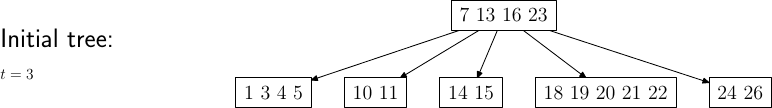
\includegraphics[width=250pt]{imagens/insertion_ex1.png}
  \label{fig_insertion_ex1}
\end{figure} 
\begin{figure}
   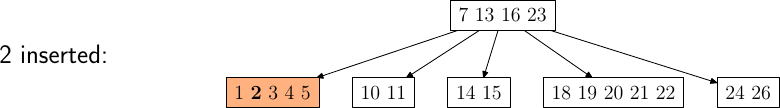
\includegraphics[width=250pt]{imagens/insertion_ex2.png}
  \label{fig_insertion_ex2}
\end{figure} 
\begin{figure}  
  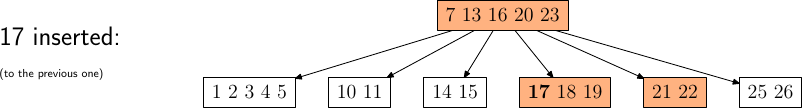
\includegraphics[width=250pt]{imagens/insertion_ex3.png}
  \label{fig_insertion_ex3}  
\end{figure} 
\end{frame}

%%%%%%%%%%%%%%%%%%%%%%%%%%%%%%%%%%%%%%%%%%%%%%%%%%%%%%%%%%%%%%%%%%%%%%%%%%%%%%%%%%%%%%%%%%%%%%%%%%%%%%%%%

\begin{frame}{Inserção}{Exemplo}
\begin{figure}[!h]
\centering
   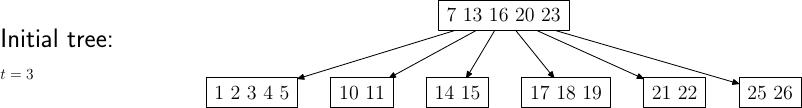
\includegraphics[width=250pt]{imagens/insertion_ex4.png}
  \label{fig_insertion_ex4}
\end{figure} 
\begin{figure}
   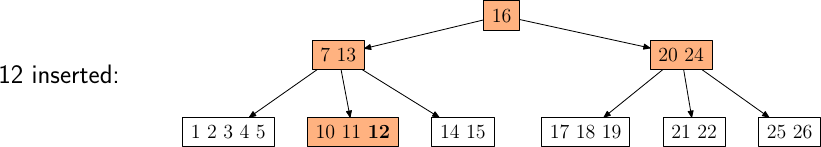
\includegraphics[width=250pt]{imagens/insertion_ex5.png}
  \label{fig_insertion_ex5}
\end{figure} 
\begin{figure}  
  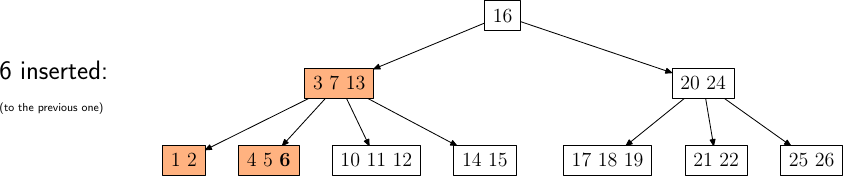
\includegraphics[width=250pt]{imagens/insertion_ex6.png}
  \label{fig_insertion_ex6}  
\end{figure} 
\end{frame}

%%%%%%%%%%%%%%%%%%%%%%%%%%%%%%%%%%%%%%%%%%%%%%%%%%%%%%%%%%%%%%%%%%%%%%%%%%%%%%%%%%%%%%%%%%%%%%%%%%%%%%%%%
\subsection{Remoção}
%%%%%%%%%%%%%%%%%%%%%%%%%%%%%%%%%%%%%%%%%%%%%%%%%%%%%%%%%%%%%%%%%%%%%%%%%%%%%%%%%%%%%%%%%%%%%%%%%%%%%%%%%

\begin{frame}{Remoção}
\begin{itemize}
 \item A remoção é similar à inserção, com adição de alguns casos especiais.
 \item Diferentemente da inserção, na remoção uma chave pode ser removida de qualquer nodo.
 \item É um procedimento mais complicado, mas com performance similar: 
 \begin{itemize}
 \item Acessos ao disco: $O(h)$.
 \item Tempo de processamento: $O(t \times h) = O(t \log_t n)$.
 \end{itemize} 
\end{itemize}
\end{frame}

%%%%%%%%%%%%%%%%%%%%%%%%%%%%%%%%%%%%%%%%%%%%%%%%%%%%%%%%%%%%%%%%%%%%%%%%%%%%%%%%%%%%%%%%%%%%%%%%%%%%%%%%%

\begin{frame}{Remoção}
\begin{itemize}
 \item Remover um nodo é feito em um único passo, partindo da raiz.
 \item Ao remover de um nodo folha:
 \begin{itemize}
 \item Caso tenha pelo menos $t$ chaves, pode-se simplesmente remover.
 \item Caso contrário, pode-se tentar movimentar chaves de um dos irmãos. 
\end{itemize}
 \item Ao remover uma chave de um nodo interno:
 \begin{itemize}
 \item Primeiramente deve-se tentar movimentar chaves de um dos filhos ou dos irmãos.
\end{itemize}
 \item Em último caso, realiza-se a operação de {\bf união} de dois nodos.
\end{itemize}
\end{frame}

%%%%%%%%%%%%%%%%%%%%%%%%%%%%%%%%%%%%%%%%%%%%%%%%%%%%%%%%%%%%%%%%%%%%%%%%%%%%%%%%%%%%%%%%%%%%%%%%%%%%%%%%%

\begin{frame}{Remoção}
Considere $k$ a chave a ser removida e $x$ o nodo que contém $k$. Existem três casos:
 \begin{enumerate}[(1)]
  \item Se a chave $k$ está em $x$, um nodo folha, e $x$ contém pelo menos $t$ chaves. 
  \begin{itemize}
  \item A remoção é trivial.
  \end{itemize}
  \item Se a chave $k$ está em $x$, um nodo interno. Existem três casos a considerar:
  \begin{enumerate}[(a)]
  \item Verifique se o filho à esquerda $y$ possui pelo menos $t$ chaves. Nesse caso, a chave predecessora $k'$ de $k$ é movida para $x$, e em seguida remove-se $k$.
  \item Simetricamente, verifique se o filho à direita $z$ possui pelo menos $t$ chaves. Nesse caso, a chave sucessora $k'$ de $k$ é movida para $x$, e em seguida remove-se $k$. 
  % \item Se o filho $y$ que precede $k$ no nodo $x$ tem no mínimo $t$ chaves (mais que o mínimo), então encontre a chave predecessora $k'$ na subárvore enraizada em $y$. Recusrivamente remova $k'$ e substitua $k$ por $k'$ em $x$.
  %\item Simetricamente, se o filho $z$ que sucede $k$ no nodo $x$ tem no mínimo $t$ chaves (mais que o mínimo), então encontre a chave sucessora $k'$ na subárvore enraizada em $z$  e substitua como no anterior.
  \item Caso contrário, se ambos $y$ e $z$  tem apenas $t-1$ chaves, realize a união de $k$.
  \begin{itemize}
  \item Todos os elementos em $z$ e em $y$ passam a pertencer a um único nodo, em conjunto com a chave $k$. 
  \item Com isso, $k$ e o ponteiro para $z$ são removidos de $x$. $y$ agora contém $2t-1$ chaves, e subsequentemente $k$ é removida.
  \end{itemize} 
  \end{enumerate} 
 \end{enumerate}
\end{frame}

%%%%%%%%%%%%%%%%%%%%%%%%%%%%%%%%%%%%%%%%%%%%%%%%%%%%%%%%%%%%%%%%%%%%%%%%%%%%%%%%%%%%%%%%%%%%%%%%%%%%%%%%%

\begin{frame}{Remoção}
 \begin{enumerate}[(3)]
  \item Se a chave $k$ não foi encontrada no nodo $x$. 
  \begin{itemize}
    \item É necessário determinar a subárvore $x.c[i]$ apropriada que deve conter $k$.
  \end{itemize}
  \begin{enumerate}[(a)]
  \item Ao determinar o filho que contém $k$, verifica-se se este possui apenas $t-1$ chaves.
  \begin{itemize}
  \item Verifique se um dos irmãos de $x.c[i]$ possui pelo menos $t$ chaves. Se possível, movimente uma chave do irmão à esquerda ou à direita para $x$.
  \item Se  $x.c[i]$ tiver filhos, verifique também se um deles possui pelo menos $t$ chaves. Nesse caso, movimente uma chave de um filho.
  \end{itemize}
  \item Caso contrário, $x.c[i]$, todos os seus filhos e irmãos contém apenas $t-1$ chaves. Dessa forma, resta apenas fazer a intercalação de $x.c[i]$ com um de seus irmãos, o que envolve mover uma chave de $x$ para baixo.
  \end{enumerate} 
 \end{enumerate}
\end{frame}

%%%%%%%%%%%%%%%%%%%%%%%%%%%%%%%%%%%%%%%%%%%%%%%%%%%%%%%%%%%%%%%%%%%%%%%%%%%%%%%%%%%%%%%%%%%%%%%%%%%%%%%%%

\begin{frame}{Exemplo}
Árvore inicial (t=2):
\begin{figure}[!h]
\centering
   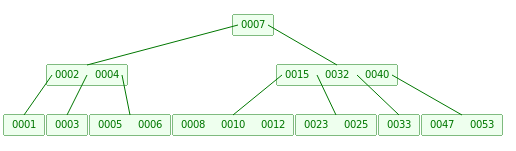
\includegraphics[width=250pt]{imagens/remocao1.png}
  \label{fig_remocao1}
\end{figure} 
\end{frame}


%%%%%%%%%%%%%%%%%%%%%%%%%%%%%%%%%%%%%%%%%%%%%%%%%%%%%%%%%%%%%%%%%%%%%%%%%%%%%%%%%%%%%%%%%%%%%%%%%%%%%%%%%

\begin{frame}{Exemplo}
Caso 1: remover 6
\begin{figure}[!h]
\centering
   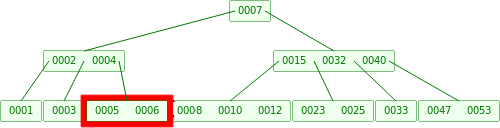
\includegraphics[width=250pt]{imagens/remocao2.png}
  \label{fig_remocao2}
\end{figure} 
Trivial, pois o nodo, que é folha, contém mais que $t-1$ chaves.
\end{frame}

%%%%%%%%%%%%%%%%%%%%%%%%%%%%%%%%%%%%%%%%%%%%%%%%%%%%%%%%%%%%%%%%%%%%%%%%%%%%%%%%%%%%%%%%%%%%%%%%%%%%%%%%%

\begin{frame}{Exemplo}
Caso 1: remover 6
\begin{figure}[!h]
\centering
   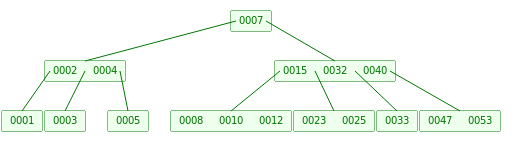
\includegraphics[width=250pt]{imagens/remocao3.png}
  \label{fig_remocao3}
\end{figure} 
Basta remover a chave.
\end{frame}

%%%%%%%%%%%%%%%%%%%%%%%%%%%%%%%%%%%%%%%%%%%%%%%%%%%%%%%%%%%%%%%%%%%%%%%%%%%%%%%%%%%%%%%%%%%%%%%%%%%%%%%%%

\begin{frame}{Exemplo}
Caso 2 (a): remover 15
\begin{figure}[!h]
\centering
   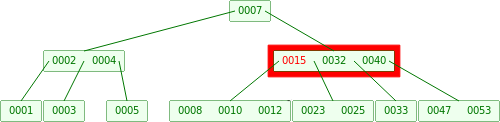
\includegraphics[width=250pt]{imagens/remocao4.png}
  \label{fig_remocao4}
\end{figure} 
Verifique se o filho à esquerda possui pelo menos $t$ chaves.
\end{frame}


%%%%%%%%%%%%%%%%%%%%%%%%%%%%%%%%%%%%%%%%%%%%%%%%%%%%%%%%%%%%%%%%%%%%%%%%%%%%%%%%%%%%%%%%%%%%%%%%%%%%%%%%%

\begin{frame}{Exemplo}
Caso 2 (a): remover 15
\begin{figure}[!h]
\centering
   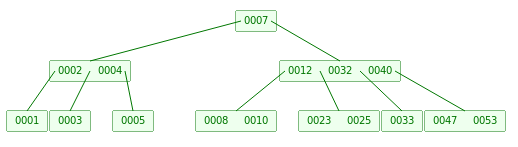
\includegraphics[width=250pt]{imagens/remocao5.png}
  \label{fig_remocao5}
\end{figure} 
Remove o 15 e o substitui pelo seu antecessor, a chave 12.
\end{frame}

%%%%%%%%%%%%%%%%%%%%%%%%%%%%%%%%%%%%%%%%%%%%%%%%%%%%%%%%%%%%%%%%%%%%%%%%%%%%%%%%%%%%%%%%%%%%%%%%%%%%%%%%%

\begin{frame}{Exemplo}
Caso 2 (b): remover 12
\begin{figure}[!h]
\centering
   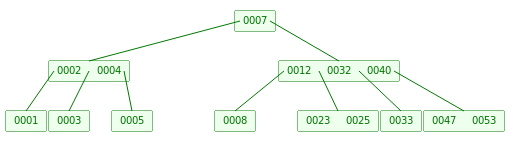
\includegraphics[width=250pt]{imagens/remocao6.png}
  \label{fig_remocao6}
\end{figure} 
Filho à esquerda possui apenas $t-1$ chaves.
\end{frame}

%%%%%%%%%%%%%%%%%%%%%%%%%%%%%%%%%%%%%%%%%%%%%%%%%%%%%%%%%%%%%%%%%%%%%%%%%%%%%%%%%%%%%%%%%%%%%%%%%%%%%%%%%

\begin{frame}{Exemplo}
Caso 2 (b): remover 12
\begin{figure}[!h]
\centering
   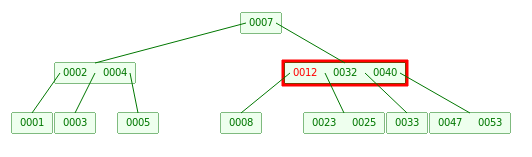
\includegraphics[width=250pt]{imagens/remocao7.png}
  \label{fig_remocao7}
\end{figure} 
Verifique se o filho à direita possui pelo menos $t$ chaves.
\end{frame}

%%%%%%%%%%%%%%%%%%%%%%%%%%%%%%%%%%%%%%%%%%%%%%%%%%%%%%%%%%%%%%%%%%%%%%%%%%%%%%%%%%%%%%%%%%%%%%%%%%%%%%%%%

\begin{frame}{Exemplo}
Caso 2 (b): remover 12
\begin{figure}[!h]
\centering
   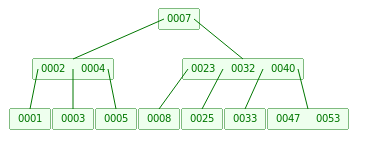
\includegraphics[width=250pt]{imagens/remocao8.png}
  \label{fig_remocao8}
\end{figure} 
Remove o 12 e o substitui pelo seu sucessor, a chave 23.
\end{frame}

%%%%%%%%%%%%%%%%%%%%%%%%%%%%%%%%%%%%%%%%%%%%%%%%%%%%%%%%%%%%%%%%%%%%%%%%%%%%%%%%%%%%%%%%%%%%%%%%%%%%%%%%%

\begin{frame}{Exemplo}
Caso 2 (c): remover 2
\begin{figure}[!h]
\centering
   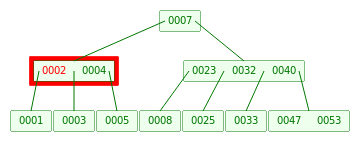
\includegraphics[width=250pt]{imagens/remocao9.png}
  \label{fig_remocao9}
\end{figure} 
Nenhum dos filhos do nodo interno com chave 2 possui mais que $t-1$ chaves
\end{frame}

%%%%%%%%%%%%%%%%%%%%%%%%%%%%%%%%%%%%%%%%%%%%%%%%%%%%%%%%%%%%%%%%%%%%%%%%%%%%%%%%%%%%%%%%%%%%%%%%%%%%%%%%%

\begin{frame}{Exemplo}
Caso 2 (c): remover 2
\begin{figure}[!h]
\centering
   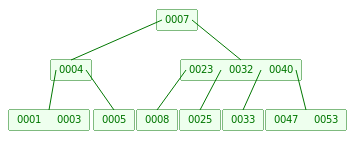
\includegraphics[width=250pt]{imagens/remocao10.png}
  \label{fig_remocao10}
\end{figure} 
A chave 2 desce e realiza-se a unidão dos filhos. Em seguida remove a chave 2.
\end{frame}

%%%%%%%%%%%%%%%%%%%%%%%%%%%%%%%%%%%%%%%%%%%%%%%%%%%%%%%%%%%%%%%%%%%%%%%%%%%%%%%%%%%%%%%%%%%%%%%%%%%%%%%%%

\begin{frame}{Exemplo}
Caso 3 (a): remover 33
\begin{figure}[!h]
\centering
   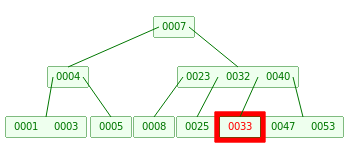
\includegraphics[width=250pt]{imagens/remocao11.png}
  \label{fig_remocao11}
\end{figure} 
O nodo que contém a chave 33 possui apenas $t-1$ chaves. O nodo não possui filhos. Verifique se um dos irmãos possui pelo menos $t$ chaves.
\end{frame}

%%%%%%%%%%%%%%%%%%%%%%%%%%%%%%%%%%%%%%%%%%%%%%%%%%%%%%%%%%%%%%%%%%%%%%%%%%%%%%%%%%%%%%%%%%%%%%%%%%%%%%%%%

\begin{frame}{Exemplo}
Caso 3 (a): remover 33
\begin{figure}[!h]
\centering
   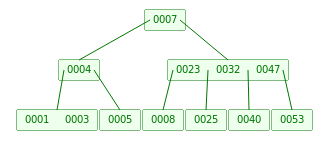
\includegraphics[width=250pt]{imagens/remocao12.png}
  \label{fig_remocao12}
\end{figure} 
Uma chave do irmão sobre e uma chave do pai desce. Em seguida, remove a chave 33.	
\end{frame}

%%%%%%%%%%%%%%%%%%%%%%%%%%%%%%%%%%%%%%%%%%%%%%%%%%%%%%%%%%%%%%%%%%%%%%%%%%%%%%%%%%%%%%%%%%%%%%%%%%%%%%%%%

\begin{frame}{Exemplo}
Caso 3 (b): remover 40
\begin{figure}[!h]
\centering
   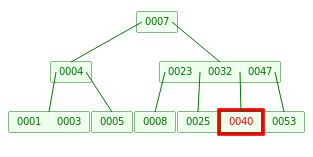
\includegraphics[width=250pt]{imagens/remocao13.png}
  \label{fig_remocao13}
\end{figure} 
Nenhum dos filhos ou irmãos possui mais que $t-1$ chaves. 
\end{frame}

%%%%%%%%%%%%%%%%%%%%%%%%%%%%%%%%%%%%%%%%%%%%%%%%%%%%%%%%%%%%%%%%%%%%%%%%%%%%%%%%%%%%%%%%%%%%%%%%%%%%%%%%%

\begin{frame}{Exemplo}
Caso 3 (b): remover 40
\begin{figure}[!h]
\centering
   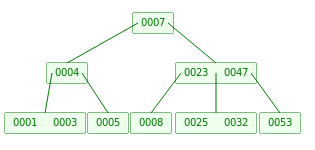
\includegraphics[width=250pt]{imagens/remocao14.png}
  \label{fig_remocao14}
\end{figure} 
Uma chave do pai desce e realiza-se a união com um dos irmãos. Em seguida, remove a chave 40.
\end{frame}

%%%%%%%%%%%%%%%%%%%%%%%%%%%%%%%%%%%%%%%%%%%%%%%%%%%%%%%%%%%%%%%%%%%%%%%%%%%%%%%%%%%%%%%%%%%%%%%%%%%%%%%%%
\section{Tipos de Árvores B}
%%%%%%%%%%%%%%%%%%%%%%%%%%%%%%%%%%%%%%%%%%%%%%%%%%%%%%%%%%%%%%%%%%%%%%%%%%%%%%%%%%%%%%%%%%%%%%%%%%%%%%%%%
\subsection{Árvore-2-3}
%%%%%%%%%%%%%%%%%%%%%%%%%%%%%%%%%%%%%%%%%%%%%%%%%%%%%%%%%%%%%%%%%%%%%%%%%%%%%%%%%%%%%%%%%%%%%%%%%%%%%%%%%

\begin{frame}{Introdução}{Árvore-2-3}
\begin{itemize}
 \item Um caso particular de Árvore B é a chamada Árvore-2-3, que {\bf não segue as regras} apresentadas em \cite{Cormen2012}.
 \item Cada nó da árvore-2-3 tem 1 ou 2 chaves.
 \begin{itemize}
 \item Consequentemente cada nodo possui 2 ou 3 filhos, daí o nome. 
 \end{itemize}
 \item A Árvore-2-3 é uma árvore usada fazer busca de dados armazenados na memória principal.
 \item Na prática, para armazenamento e busca em disco, uma árvore B usa uma ordem $t$ grande, tipicamente de alguma centenas de chaves.
\end{itemize}
\end{frame}

%%%%%%%%%%%%%%%%%%%%%%%%%%%%%%%%%%%%%%%%%%%%%%%%%%%%%%%%%%%%%%%%%%%%%%%%%%%%%%%%%%%%%%%%%%%%%%%%%%%%%%%%%

\begin{frame}{Exemplo}
\begin{figure}[!h]
\centering
   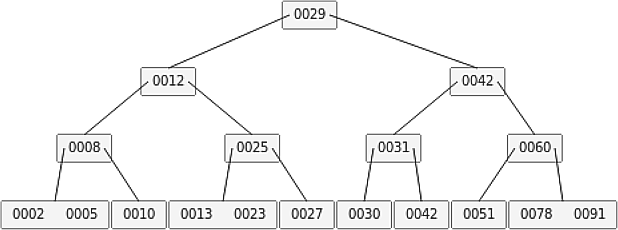
\includegraphics[width=250pt]{imagens/arvore-2-3.png}
  \label{fig_arvore-2-3}
\end{figure} 
\end{frame}

%%%%%%%%%%%%%%%%%%%%%%%%%%%%%%%%%%%%%%%%%%%%%%%%%%%%%%%%%%%%%%%%%%%%%%%%%%%%%%%%%%%%%%%%%%%%%%%%%%%%%%%%%
\subsection{Árvore-2-3-4}
%%%%%%%%%%%%%%%%%%%%%%%%%%%%%%%%%%%%%%%%%%%%%%%%%%%%%%%%%%%%%%%%%%%%%%%%%%%%%%%%%%%%%%%%%%%%%%%%%%%%%%%%%

\begin{frame}{Introdução}{Árvore-2-3-4}
\begin{itemize}
 \item Um caso particular de Árvore B é a chamada árvore-2-3-4.
 \item Segundo a definição de \cite{Cormen2012}, é a menor árvore B possível.
 \item Uma árvore-2-3-4 é uma Árvore B de ordem $t = 2$.
 \item Cada nó da árvore-2-3-4 tem 1, 2 ou 3 chaves.
 \item Cada nó da árvore-2-3-4 tem 2, 3 ou 4 filhos, daí o nome.
\end{itemize}
\end{frame}

%%%%%%%%%%%%%%%%%%%%%%%%%%%%%%%%%%%%%%%%%%%%%%%%%%%%%%%%%%%%%%%%%%%%%%%%%%%%%%%%%%%%%%%%%%%%%%%%%%%%%%%%%

\begin{frame}{Exemplo}
\begin{figure}[!h]
\centering
   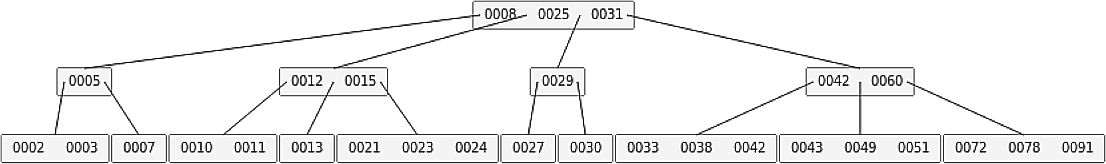
\includegraphics[width=350pt]{imagens/arvore-2-3-4.png}
  \label{fig_arvore-2-3-4}
\end{figure} 
\end{frame}


%%%%%%%%%%%%%%%%%%%%%%%%%%%%%%%%%%%%%%%%%%%%%%%%%%%%%%%%%%%%%%%%%%%%%%%%%%%%%%%%%%%%%%%%%%%%%%%%%%%%%%%%%

\begin{frame}{Conclusão}

\begin{figure}[!h]
  \centering
  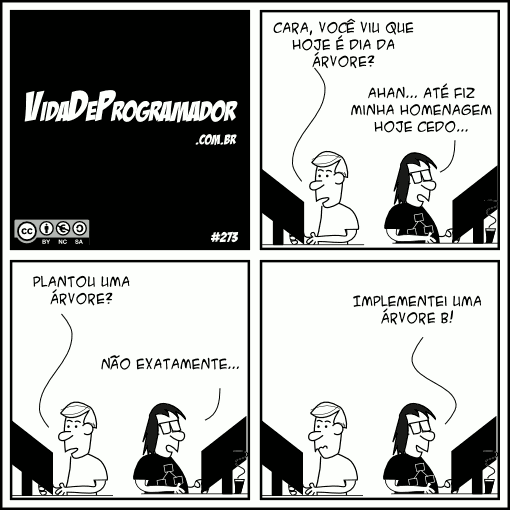
\includegraphics[width=150pt]{imagens/tirinha273.png}
  \label{fig_tirinha}
\end{figure}
\end{frame}

%%%%%%%%%%%%%%%%%%%%%%%%%%%%%%%%%%%%%%%%%%%%%%%%%%%%%%%%%%%%%%%%%%%%%%%%%%%%%%%%%%%%%%%%%%%%%%%%%%%%%%%%%
%
%\begin{frame}
%\Huge{\centerline{Dúvidas?}}
%
%\begin{figure}[!h]
%  \centering
%  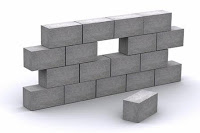
\includegraphics[width=100pt]{imagens/duvidas.jpg}
%  \label{fig_fim}
%\end{figure}
%\end{frame}


%%%%%%%%%%%%%%%%%%%%%%%%%%%%%%%%%%%%%%%%%%%%%%%%%%%%%%%%%%%%%%%%%%%%%%%%%%%%%%%%%%%%%%%%%%%%%%%%%%%%%%%%%
 
\section{Referências bibliográficas}
  \frame{\frametitle{Referências Bibliográficas}
    \bibliographystyle{abntex2-alf}
    \bibliography{referencias}
 }
  

%%%%%%%%%%%%%%%%%%%%%%%%%%%%%%%%%%%%%%%%%%%%%%%%%%%%%%%%%%%%%%%%%%%%%%%%%%%%%%%%%%%%%%%%%%%%%%%%%%%%%%%%%

\begin{frame}{Material Complementar}
Animações
\begin{itemize}
\item \href{https://www.cs.usfca.edu/~galles/visualization/BTree.html}{https://www.cs.usfca.edu/~galles/visualization/BTree.html}
\begin{itemize}
\item Obs.: Escolha "Max Degree = 4" para árvore de ordem $t=2$.
\end{itemize}
\item \href{http://cs.armstrong.edu/liang/animation/web/24Tree.html}{http://cs.armstrong.edu/liang/animation/web/24Tree.html}
\begin{itemize}
\item Árvore 2-3-4
\end{itemize}
\end{itemize}
\end{frame}

%%%%%%%%%%%%%%%%%%%%%%%%%%%%%%%%%%%%%%%%%%%%%%%%%%%%%%%%%%%%%%%%%%%%%%%%%%%%%%%%%%%%%%%%%%%%%%%%%%%%%%%%%

\end{document} 